\chapter{Smart Contracts and Custom Blockchain}\label{ch:contracts}

This chapter presents the complete implementation of our smart contract layer and custom Go blockchain. We analyze each contract in detail---state variables, events, modifiers, and functions---then describe the custom blockchain architecture including EVM embedding, gasless execution, REST API, PBFT consensus, and BoltDB persistence.

\section{Smart Contract Overview}

Four Solidity contracts compose the election logic, deployed in strict dependency order:

\begin{figure}[H]
\centering
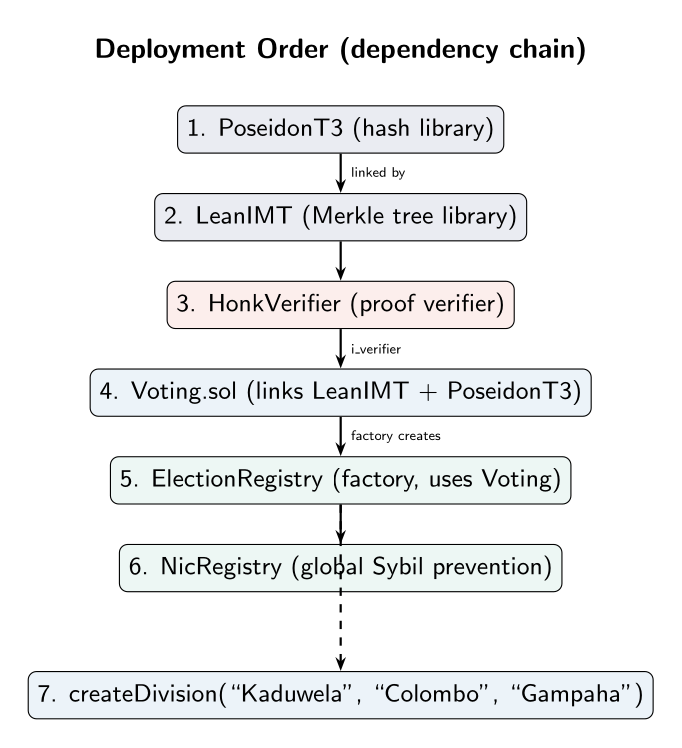
\includegraphics[width=0.85\textwidth]{Images/fig_deploy_order.png}
\caption{Contract deployment order showing dependencies: HonkVerifier must exist before Voting, which must exist before ElectionRegistry can create divisions.}
\label{fig:deploy-order}
\end{figure}

\section{Voting.sol: Per-Division Election State Machine}

\texttt{Voting.sol} is the core contract implementing a complete election lifecycle for a single polling division.

\subsection{State Variables}

\begin{lstlisting}[language=Java, caption={Voting.sol state variable declarations.}]
// Immutables (set at construction)
IHonkVerifier private immutable i_verifier;

// Constants
uint256 public constant MAX_CANDIDATES = 100;

// Administration
address public s_gnOfficer;
string public s_question;
string[] public s_candidates;

// Phase management
uint256 public s_registrationEndTime;
uint256 public s_votingEndTime;
Phase public s_phase;

// Per-election state (keyed by electionId)
uint256 public s_electionId;
mapping(uint256 => mapping(address => bool)) public s_voters;
mapping(uint256 => mapping(address => bool)) public s_hasRegistered;
mapping(uint256 => mapping(uint256 => bool)) public s_commitments;
mapping(uint256 => mapping(bytes32 => bool)) public s_nullifierHashes;
mapping(uint256 => mapping(uint256 => uint256)) public s_voteCounts;
mapping(uint256 => IncrementalTreeData) internal s_trees;
\end{lstlisting}

\subsection{Events}

\begin{lstlisting}[language=Java, caption={Voting.sol event declarations.}]
event VoterAdded(address indexed voter);
event GNOfficerUpdated(address indexed gnOfficer);
event NewLeaf(uint256 index, uint256 value);
event QuestionUpdated(string question);
event CandidatesUpdated(string[] candidates);
event PhaseChanged(Phase indexed phase, uint256 deadline);
event ElectionReset(uint256 indexed electionId);
event VoteCast(
    bytes32 nullifierHash,
    address voter,
    uint256 candidate,
    uint256 timestamp,
    uint256 newCount
);
\end{lstlisting}

\subsection{Custom Errors}

Gas-efficient custom errors replace \texttt{require} strings:

\begin{lstlisting}[language=Java, caption={Custom error declarations for precise revert reasons.}]
error CommitmentAlreadyAdded(uint256 commitment);
error NullifierHashAlreadyUsed(bytes32 nullifierHash);
error InvalidProof();
error NotAllowedToVote();
error EmptyTree();
error InvalidRoot();
error WrongPhase(Phase expected, Phase actual);
error InvalidCandidate(uint256 index);
error InvalidDuration();
error TooManyCandidates(uint256 provided, uint256 max);
error NoCandidates();
\end{lstlisting}

\subsection{Modifiers}

\begin{lstlisting}[language=Java, caption={Phase enforcement and access control modifiers.}]
modifier inPhase(Phase expected) {
    _maybeAdvancePhase();  // Auto-advance if deadline passed
    if (s_phase != expected)
        revert WrongPhase(expected, s_phase);
    _;
}

modifier onlyOwnerOrGN() {
    if (msg.sender != owner() && msg.sender != s_gnOfficer)
        revert OwnableUnauthorizedAccount(msg.sender);
    _;
}
\end{lstlisting}

The \texttt{\_maybeAdvancePhase()} internal function checks block timestamps against stored deadlines and advances the phase accordingly, ensuring consistent behavior regardless of when transactions arrive.

\subsection{Registration Function}

\begin{lstlisting}[language=Java, caption={Voter registration: commitment insertion into Merkle tree.}]
function register(uint256 _commitment) 
    external inPhase(Phase.Registration) 
{
    uint256 eid = s_electionId;
    
    // Check 1: Voter is on the allowlist
    if (!s_voters[eid][msg.sender])
        revert NotAllowedToVote();
    
    // Check 2: Voter hasn't already registered
    if (s_hasRegistered[eid][msg.sender])
        revert NotAllowedToVote();
    
    // Check 3: Commitment is unique
    if (s_commitments[eid][_commitment])
        revert CommitmentAlreadyAdded(_commitment);
    
    // Insert into Merkle tree (LeanIMT)
    uint256 leafIndex = LeanIMT._insert(
        s_trees[eid], _commitment
    );
    
    // Update state
    s_hasRegistered[eid][msg.sender] = true;
    s_commitments[eid][_commitment] = true;
    
    emit NewLeaf(leafIndex, _commitment);
}
\end{lstlisting}

\subsection{Vote Function}

\begin{lstlisting}[language=Java, caption={Anonymous vote casting with ZK proof verification.}]
function vote(
    bytes memory _proof,
    bytes32 _nullifierHash,
    bytes32 _root,
    bytes32 _vote,
    bytes32 _depth
) external inPhase(Phase.Voting) {
    uint256 eid = s_electionId;
    uint256 candidateIdx = uint256(_vote);
    
    // Check 1: Valid candidate index
    if (candidateIdx >= s_candidates.length)
        revert InvalidCandidate(candidateIdx);
    
    // Check 2: Root matches current tree
    if (s_trees[eid]._root() == 0)
        revert EmptyTree();
    if (bytes32(s_trees[eid]._root()) != _root)
        revert InvalidRoot();
    
    // Check 3: Verify ZK proof
    bytes32[] memory publicInputs = new bytes32[](4);
    publicInputs[0] = _nullifierHash;
    publicInputs[1] = _root;
    publicInputs[2] = _vote;
    publicInputs[3] = _depth;
    
    if (!i_verifier.verify(_proof, publicInputs))
        revert InvalidProof();
    
    // Check 4: Nullifier not already used
    if (s_nullifierHashes[eid][_nullifierHash])
        revert NullifierHashAlreadyUsed(_nullifierHash);
    
    // State updates
    s_nullifierHashes[eid][_nullifierHash] = true;
    s_voteCounts[eid][candidateIdx]++;
    
    emit VoteCast(
        _nullifierHash, msg.sender, candidateIdx,
        block.timestamp,
        s_voteCounts[eid][candidateIdx]
    );
}
\end{lstlisting}

\begin{figure}[H]
\centering
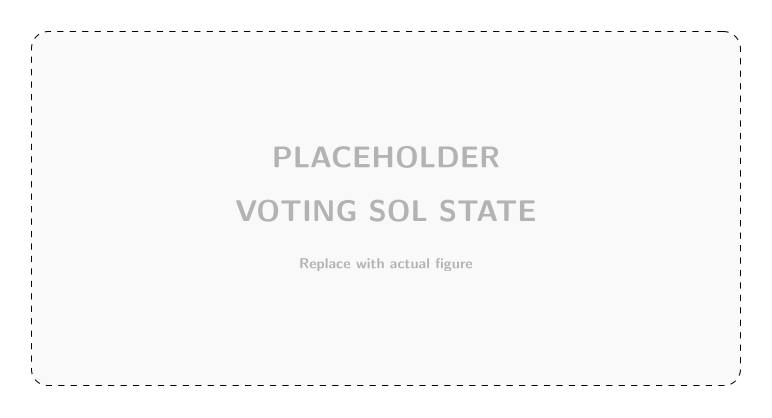
\includegraphics[width=0.85\textwidth]{Images/fig_voting_sol_state.png}
\caption{Voting.sol internal state machine with five verification checks during the vote function.}
\label{fig:voting-state-detail}
\end{figure}

\subsection{View Functions}

\begin{lstlisting}[language=Java, caption={Key view functions for state querying.}]
function getVotingData() external view returns (
    string memory question,
    address owner_addr,
    Phase phase,
    uint256 regEndTime,
    uint256 votEndTime,
    uint256 treeSize,
    uint256 depth,
    uint256 root,
    uint256 candidateCount
) {
    uint256 eid = s_electionId;
    return (
        s_question, owner(), _currentPhase(),
        s_registrationEndTime, s_votingEndTime,
        LeanIMT._size(s_trees[eid]),
        LeanIMT._depth(s_trees[eid]),
        s_trees[eid]._root(),
        s_candidates.length
    );
}

function isNullifierUsed(bytes32 _hash) 
    external view returns (bool) 
{
    return s_nullifierHashes[s_electionId][_hash];
}
\end{lstlisting}

\section{ElectionRegistry.sol: Factory Pattern and Aggregation}

\begin{figure}[H]
\centering
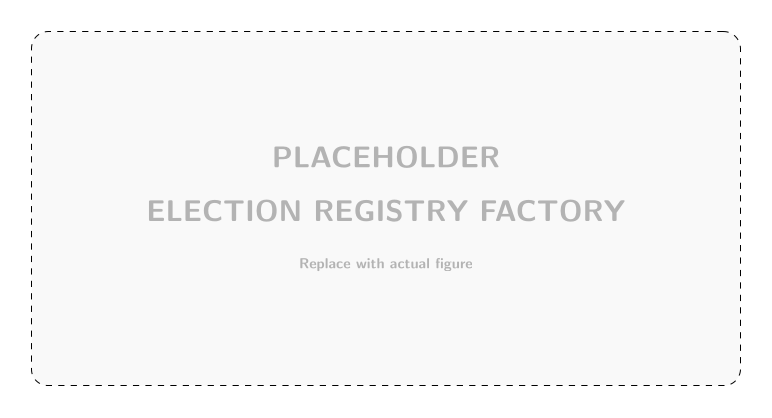
\includegraphics[width=0.85\textwidth]{Images/fig_election_registry_factory.png}
\caption{ElectionRegistry factory pattern: creates and manages 160 independent Voting contract instances with national result aggregation.}
\label{fig:registry-factory}
\end{figure}

\subsection{Division Structure}

\begin{lstlisting}[language=Java, caption={Division struct and state in ElectionRegistry.}]
struct Division {
    string name;              // e.g., "Kaduwela", "Colombo North"
    address votingContract;   // Deployed Voting.sol address
    address gnOfficer;        // Assigned GN officer
    bool active;              // Can be deactivated
}

Division[] public divisions;
address public immutable i_verifier;  // Shared HonkVerifier
\end{lstlisting}

\subsection{Factory Methods}

\begin{lstlisting}[language=Java, caption={Division creation via factory pattern.}]
function createDivision(string calldata name) 
    external onlyOwner 
    returns (uint256 divisionId, address votingContract)
{
    // Deploy fresh Voting instance with shared verifier
    Voting newVoting = new Voting(
        IHonkVerifier(i_verifier), msg.sender
    );
    
    divisions.push(Division({
        name: name,
        votingContract: address(newVoting),
        gnOfficer: address(0),
        active: true
    }));
    
    divisionId = divisions.length - 1;
    votingContract = address(newVoting);
    
    emit DivisionCreated(divisionId, name, votingContract);
}
\end{lstlisting}

\subsection{National Aggregation}

\begin{lstlisting}[language=Java, caption={National vote count aggregation across all active divisions.}]
function getNationalResults() 
    external view returns (uint256[] memory totals)
{
    // Determine max candidates across all divisions
    uint256 maxCandidates = 0;
    for (uint256 i = 0; i < divisions.length; i++) {
        if (!divisions[i].active) continue;
        uint256 count = Voting(divisions[i].votingContract)
            .getCandidates().length;
        if (count > maxCandidates) maxCandidates = count;
    }
    
    // Sum votes per candidate across all divisions
    totals = new uint256[](maxCandidates);
    for (uint256 i = 0; i < divisions.length; i++) {
        if (!divisions[i].active) continue;
        uint256[] memory divVotes = Voting(
            divisions[i].votingContract
        ).getVoteCounts();
        for (uint256 c = 0; c < divVotes.length; c++) {
            totals[c] += divVotes[c];
        }
    }
}
\end{lstlisting}

\section{NicRegistry.sol: Cross-Division Sybil Prevention}

\begin{figure}[H]
\centering
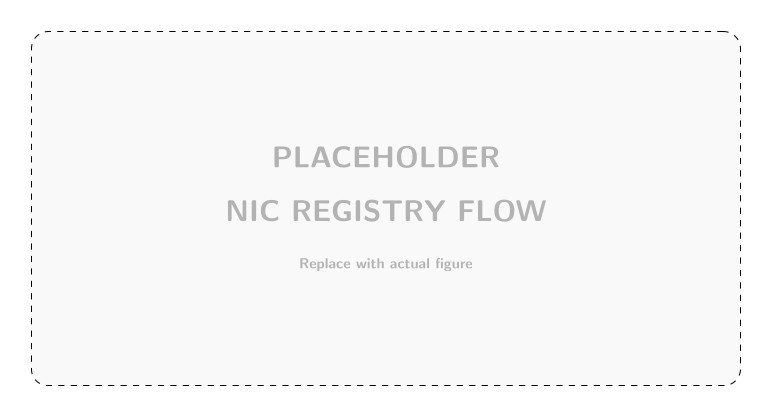
\includegraphics[width=0.85\textwidth]{Images/fig_nic_registry_flow.png}
\caption{NicRegistry flow: hashed NIC reservation prevents the same citizen from registering across multiple polling divisions.}
\label{fig:nic-flow}
\end{figure}

\subsection{Design Rationale}

A voter could potentially register in multiple divisions using different wallets. The NicRegistry prevents this by storing hashed National Identity Card numbers:

\begin{equation}
\text{nicHash} = \Poseidon(\text{NIC\_number}, \text{SERVER\_PEPPER})
\end{equation}

The server pepper is a secret known only to the election authority, preventing brute-force enumeration of NIC hashes from the public blockchain state.

\begin{lstlisting}[language=Java, caption={NicRegistry contract for cross-division Sybil prevention.}]
contract NicRegistry is Ownable {
    mapping(bytes32 => bool) private s_usedNicHashes;
    mapping(address => bool) private s_votingContracts;
    
    error NicRegistry__AlreadyUsed(bytes32 nicHash);
    event NicHashReserved(bytes32 indexed nicHash);
    
    function setVotingContract(
        address votingContract, bool authorized
    ) external onlyOwner {
        s_votingContracts[votingContract] = authorized;
    }
    
    function reserveNicHash(
        bytes32 nicHash, address votingContract
    ) external returns (bool) {
        // Only owner or GN of specified division can reserve
        require(
            msg.sender == owner() || 
            _isGNOf(msg.sender, votingContract),
            "Unauthorized"
        );
        
        if (s_usedNicHashes[nicHash])
            revert NicRegistry__AlreadyUsed(nicHash);
        
        s_usedNicHashes[nicHash] = true;
        emit NicHashReserved(nicHash);
        return true;
    }
}
\end{lstlisting}

\section{HonkVerifier.sol: Auto-Generated Proof Verifier}

The HonkVerifier is auto-generated by the Barretenberg compiler and contains:
\begin{itemize}
    \item Hardcoded verification key (circuit-specific polynomial commitments)
    \item Proof deserialization logic
    \item Fiat--Shamir transcript reconstruction
    \item BN254 pairing verification using precompile \texttt{0x08}
\end{itemize}

\begin{lstlisting}[language=Java, caption={HonkVerifier interface and key constants.}]
interface IHonkVerifier {
    function verify(
        bytes calldata _proof, 
        bytes32[] calldata _publicInputs
    ) external view returns (bool);
}

// Internal constants (from verification key)
uint256 constant N = 32768;
uint256 constant LOG_N = 15;
uint256 constant NUMBER_OF_PUBLIC_INPUTS = 4;
// Public inputs order: [nullifierHash, root, vote, depth]
\end{lstlisting}

\section{Deployment Pipeline}

The contracts must be deployed in strict dependency order:

\begin{enumerate}
    \item \texttt{PoseidonT3} library (used by LeanIMT)
    \item \texttt{LeanIMT} library (linked into Voting)
    \item \texttt{HonkVerifier} (standalone, no dependencies)
    \item \texttt{Voting} (references HonkVerifier address)
    \item \texttt{ElectionRegistry} (references HonkVerifier, deploys Voting instances)
    \item \texttt{NicRegistry} (standalone, references Voting contracts post-deploy)
\end{enumerate}

Library linking is required because Solidity libraries with external functions must be deployed separately and their addresses embedded in the calling contract's bytecode at deploy time.

\section{Custom Go Blockchain Architecture}

\begin{figure}[H]
\centering
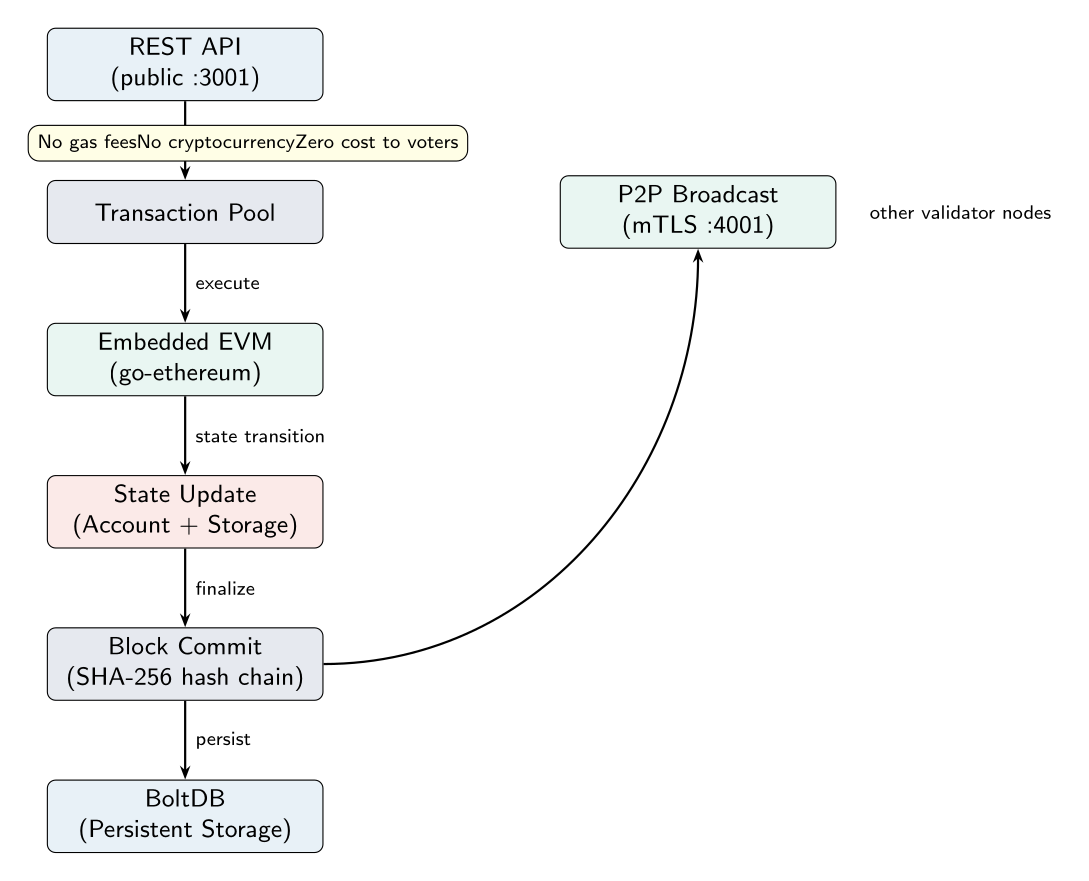
\includegraphics[width=0.85\textwidth]{Images/fig_go_blockchain.png}
\caption{Custom Go blockchain architecture showing the six internal packages and their interactions.}
\label{fig:go-blockchain}
\end{figure}

\subsection{Package Organization}

\begin{table}[H]
\centering
\caption{Go blockchain internal package structure.}
\label{tab:go-packages}
\begin{tabular}{|l|p{8cm}|}
\hline
\textbf{Package} & \textbf{Responsibility} \\
\hline
\texttt{internal/core} & Blockchain data structures: Transaction, Block, Blockchain types \\
\hline
\texttt{internal/evm} & Embedded go-ethereum EVM: StateDB, contract execution, precompiles \\
\hline
\texttt{internal/api} & HTTP handlers, middleware, routing (public + P2P listeners) \\
\hline
\texttt{internal/network} & Peer discovery, mTLS broadcast, periodic state synchronization \\
\hline
\texttt{internal/persistence} & BoltDB on-disk block and state storage \\
\hline
\texttt{internal/security} & RSA admin authentication, mTLS certificate management \\
\hline
\end{tabular}
\end{table}

\subsection{Gasless Execution Model}

\begin{lstlisting}[language=Java, caption={Gasless EVM execution in Go (simplified).}]
func (e *EVMExecutor) ExecuteCall(
    from, to common.Address,
    data []byte,
) ([]byte, error) {
    // Set gas limit but never deduct cost
    gasLimit := uint64(16_000_000)
    
    // Create EVM with current state
    evm := vm.NewEVM(
        e.blockContext(),
        vm.TxContext{Origin: from},
        e.stateDB,
        e.chainConfig,
        vm.Config{},
    )
    
    // Execute (gas metered for DoS protection only)
    ret, remainingGas, err := evm.Call(
        vm.AccountRef(from), to, data, gasLimit,
        new(uint256.Int), // value = 0 (gasless)
    )
    
    // Commit state changes (no gas deduction)
    e.stateDB.Commit()
    return ret, err
}
\end{lstlisting}

\subsection{Block Structure}

\begin{lstlisting}[language=Java, caption={Block and Transaction structures in Go.}]
type Transaction struct {
    ID        string    `json:"id"`
    Type      string    `json:"type"`      // "register", "vote", "admin"
    From      string    `json:"from"`
    To        string    `json:"to"`
    Data      []byte    `json:"data"`
    Timestamp time.Time `json:"timestamp"`
}

type Block struct {
    Index        uint64        `json:"index"`
    Timestamp    time.Time     `json:"timestamp"`
    Transactions []Transaction `json:"transactions"`
    PrevHash     string        `json:"prev_hash"`
    Hash         string        `json:"hash"`
    Validator    string        `json:"validator"`
}
\end{lstlisting}

\section{REST API Specification}

\begin{figure}[H]
\centering
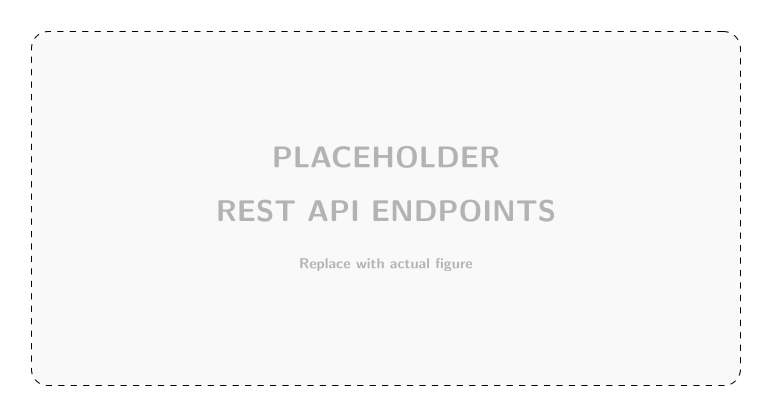
\includegraphics[width=0.85\textwidth]{Images/fig_rest_api_endpoints.png}
\caption{REST API endpoint map showing public (read), voter (rate-limited), and admin (RSA-signed) categories.}
\label{fig:rest-api}
\end{figure}

\subsection{Public Read Endpoints}

\begin{table}[H]
\centering
\caption{Public API endpoints (no authentication required).}
\label{tab:public-api}
\begin{tabular}{|l|l|p{5cm}|}
\hline
\textbf{Method} & \textbf{Endpoint} & \textbf{Response} \\
\hline
GET & \texttt{/voting-data} & Current election state, phases, tree info \\
\hline
GET & \texttt{/candidates} & Candidate name array \\
\hline
GET & \texttt{/vote-counts} & Per-candidate vote tallies \\
\hline
GET & \texttt{/voter/\{id\}} & Voter allowlist and registration status \\
\hline
GET & \texttt{/commitments} & All registered commitments (Merkle leaves) \\
\hline
GET & \texttt{/chain} & Full blockchain (all blocks) \\
\hline
GET & \texttt{/blocks?page=\&limit=} & Paginated block history \\
\hline
GET & \texttt{/health} & Node health status \\
\hline
\end{tabular}
\end{table}

\subsection{Voter Endpoints (Rate Limited)}

Rate limited to 1 request/second with burst of 5:

\begin{table}[H]
\centering
\caption{Voter-facing endpoints with rate limiting.}
\label{tab:voter-api}
\begin{tabular}{|l|l|p{5cm}|}
\hline
\textbf{Method} & \textbf{Endpoint} & \textbf{Action} \\
\hline
POST & \texttt{/register} & Submit commitment for Merkle tree insertion \\
\hline
POST & \texttt{/vote} & Submit ZK proof and anonymous vote \\
\hline
\end{tabular}
\end{table}

\subsection{Admin Endpoints (RSA Authenticated)}

\begin{table}[H]
\centering
\caption{Admin API endpoints requiring RSA signature authentication.}
\label{tab:admin-api}
\begin{tabular}{|l|l|p{5cm}|}
\hline
\textbf{Method} & \textbf{Endpoint} & \textbf{Action} \\
\hline
POST & \texttt{/add-voter} & Add voter to allowlist \\
\hline
POST & \texttt{/set-question} & Set ballot question \\
\hline
POST & \texttt{/set-candidates} & Set candidate list \\
\hline
POST & \texttt{/start-registration} & Begin registration phase \\
\hline
POST & \texttt{/start-voting} & Begin voting phase \\
\hline
POST & \texttt{/end-election} & End election early \\
\hline
POST & \texttt{/reset-election} & Reset to setup phase \\
\hline
\end{tabular}
\end{table}

\section{Admin RSA Authentication}

\begin{lstlisting}[language=Java, caption={RSA signature verification for admin endpoints.}]
// Admin request authentication:
// Header: X-Admin-Signature = base64(RSA-SHA256(message))
// Header: X-Admin-Timestamp = unix_seconds
// Message = "<timestamp>\n<path>\n<body>"
// Time window: +/- 5 minutes

func verifyAdminSignature(r *http.Request) error {
    sig := r.Header.Get("X-Admin-Signature")
    ts := r.Header.Get("X-Admin-Timestamp")
    
    // Check timestamp within 5-minute window
    reqTime, _ := strconv.ParseInt(ts, 10, 64)
    if abs(time.Now().Unix()-reqTime) > 300 {
        return errors.New("timestamp expired")
    }
    
    // Reconstruct signed message
    body, _ := io.ReadAll(r.Body)
    message := fmt.Sprintf("%s\n%s\n%s", ts, r.URL.Path, body)
    
    // Verify RSA-SHA256 PKCS#1 v1.5 signature
    hash := sha256.Sum256([]byte(message))
    return rsa.VerifyPKCS1v15(adminPubKey, crypto.SHA256, hash[:], sigBytes)
}
\end{lstlisting}

\section{PBFT Consensus}

\begin{figure}[H]
\centering
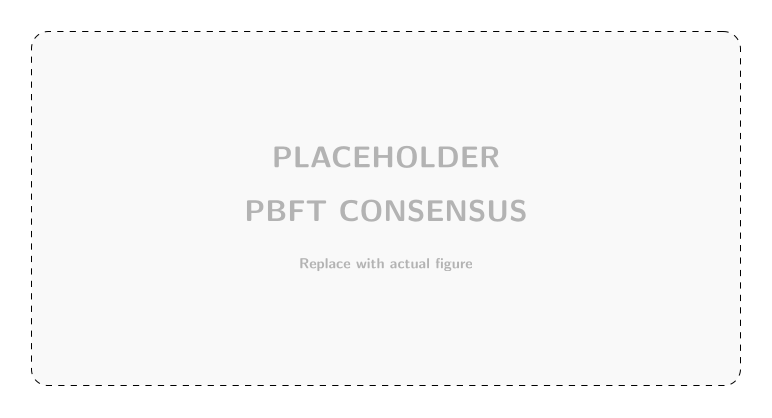
\includegraphics[width=0.85\textwidth]{Images/fig_pbft_consensus.png}
\caption{PBFT consensus flow among election commission validator nodes: pre-prepare, prepare, commit phases.}
\label{fig:pbft}
\end{figure}

Our PBFT implementation provides:
\begin{itemize}
    \item \textbf{Fault tolerance}: Tolerates $f < n/3$ Byzantine nodes
    \item \textbf{Deterministic finality}: No block reorgs possible
    \item \textbf{Geographic distribution}: Nodes in different election commission offices
    \item \textbf{mTLS communication}: All inter-node traffic encrypted and authenticated
\end{itemize}

\section{BoltDB Persistence}

\begin{lstlisting}[language=Java, caption={BoltDB block persistence layer.}]
// Buckets:
// "blocks"     -> block_index (uint64 BE) -> Block JSON
// "state"      -> "latest_index" -> uint64
// "accounts"   -> address -> Account JSON
// "storage"    -> address+slot -> value

func (p *Persistence) StoreBlock(block *Block) error {
    return p.db.Update(func(tx *bolt.Tx) error {
        b := tx.Bucket([]byte("blocks"))
        key := uint64ToBytes(block.Index)
        data, _ := json.Marshal(block)
        return b.Put(key, data)
    })
}
\end{lstlisting}

\begin{figure}[H]
\centering
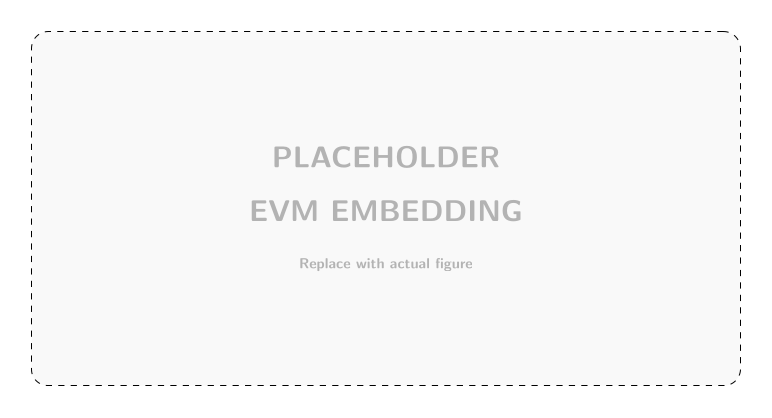
\includegraphics[width=0.85\textwidth]{Images/fig_evm_embedding.png}
\caption{EVM embedding architecture: Go blockchain wraps go-ethereum's VM package with a custom StateDB backed by BoltDB.}
\label{fig:evm-embed}
\end{figure}

\section{Summary}

This chapter has presented the complete smart contract layer (Voting.sol, ElectionRegistry.sol, NicRegistry.sol, HonkVerifier.sol) and custom Go blockchain implementation. The contracts implement a rigorous state machine with five-layer fraud prevention, while the blockchain provides gasless execution, PBFT consensus, and RSA-authenticated administration. Together, they form the trusted execution layer that our application interfaces (Chapter~\ref{ch:applications}) interact with through well-defined APIs.
